% !TeX root = ../tesis.tex

\chapter*{Introducción}
\addcontentsline{toc}{chapter}{\protect\numberline{}Introducción}
\label{chapter:Motivacion}
\vspace*{.5em}
%Presentación
%Objetivo

%Motivación
Las propiedades físicas de los materiales dependen en general del tamaño del sistema \cite{boverhof2015comparative}, por ejemplo, a escala nanom\'etrica ---de $1$ a $100$ nm \cite{boverhof2015comparative}---, la respuesta electromagn\'etica (EM) de bulto de los metales es menos relevante que los efectos de superficie \cite{zhao2008methods}.  La \emph{nanoplasm\'onica} estudia la respuesta EM a esta escala y el inter\'es en su estudio se ha renovado debido a las posibles aplicaciones que emplean las resonancias plasm\'onicas de superficie (Surface Plasmon Resonances, SPRs), como la espectroscop\'ia \cite{novotny2006principles}, el sensado \cite{jain2008noble}, la litograf\'ia \cite{stockman2011nanoplasmonics}, la biolog\'ia y  medicina \cite{jain2008noble}. Otro ejemplo donde la nanoplasmónica ha impactado es en el área de los \textit{biosensores} \cite{estevez2014trends,mun2015nanobiosensors}, definidos como ``dispositivos [$\ldots$] basados en elementos de reconocimiento biológico conectados a un transductor de señal, que relaciona la concentración de [uno o varios analítos] a una señal medible'' \cite{mun2015nanobiosensors}\index{Biosensor}. Los biosensores se clasifican según el método de reconocimiento del analito, o bien, del transductor empleado \cite{mun2015nanobiosensors}. Dentro de los biosensores comerciales, los ópticos se caracterizan por su estabilidad, por la posibilidad de mediciones sin marcadores, y por su capacidad de miniaturización y de multiplexeo \cite{estevez2014trends}, sobre todo los que se basan en nanoestructuras plasmónicas.

Los plasmones son oscilaciones colectivas de los electrones libres en un material metálico,  resultado del  acoplamiento con la radiaci\'on EM a las frecuencias en las que ocurren las SPRs \cite{stockman2011nanoplasmonics}.  Los plasmones pueden excitarse dentro de un metal (plasmones de volumen) o  sobre la superficie de alguna estructura metálica (plasmones de superficie) \cite{maier2007plasmonics}, en cuyo caso, los plasmones pueden ser de dos tipos: propagantes y localizados.  Cuando el plasmón se propaga a lo largo de una interfaz plana entre un medio diel\'ectrico y uno met\'alico se le denomina  \emph{plasm\'on-polarit\'on de superficie} (Surface Plasmon Polariton, SPP) \cite{maier2007plasmonics}.  Si el plasmón, en cambio, se encuentra en la superficie de una partícula  met\'alica, de tamaño finito, se le conoce como \emph{resonancia de plasm\'on de superficie localizado} (Localized Surface Plasmon Resonance, LSPR) \cite{maier2007plasmonics}.

Los biosensores ópticos emplean las SPRs por la respuesta que tienen ante cambios del índice de refracción de la matriz \cite{kabashin2009plasmonic}, que es el medio que rodea la estructura metálica, ya sean NPs o películas continuas.  Los sensores comerciales se caracterizan por el uso de SPPs \cite{estevez2014trends} en una configuración de reflexión total atenuada (Attenuated Total Reflection, ATR), en donde el índice de refracción del medio donde incide la luz que ilumina a la estructura metálica es mayor al de la matriz [ver Fig.  \ref{fig:ATR1}]\index{Biosensor!comercial|seealso{Plasmón polaritón de superficie (SPP)}}.  Las mediciones de reflectancia, en un sistema en configuración ATR, presentan mínimos para determinadas combinaciones de  ángulos de incidencia $\theta_i$ y longitud de onda $\lambda$  \cite{danilov2018ultra}.  Los sensores basados en las LSPRs [ver Fig. \ref{sfig:ATRNP}] han sido propuestos por algunos autores como mejora sobre ciertos sensores comerciales \cite{jain2008noble,kabashin2009plasmonic},  debido a que las LSPRs reducen el área de sensado a las dimensiones de la NP y, al poder ser excitados con iluminación directa, permiten miniaturizar el arreglo experimental empleado \cite{estevez2014trends}.



	\begin{figure}[h!]\vspace{1em}\centering
	\begin{subfigure}{.05\textwidth}\vspace{-3.5cm}\caption{}\label{sfig:ATRfilm}\end{subfigure}
	\begin{subfigure}{.43\textwidth} 
		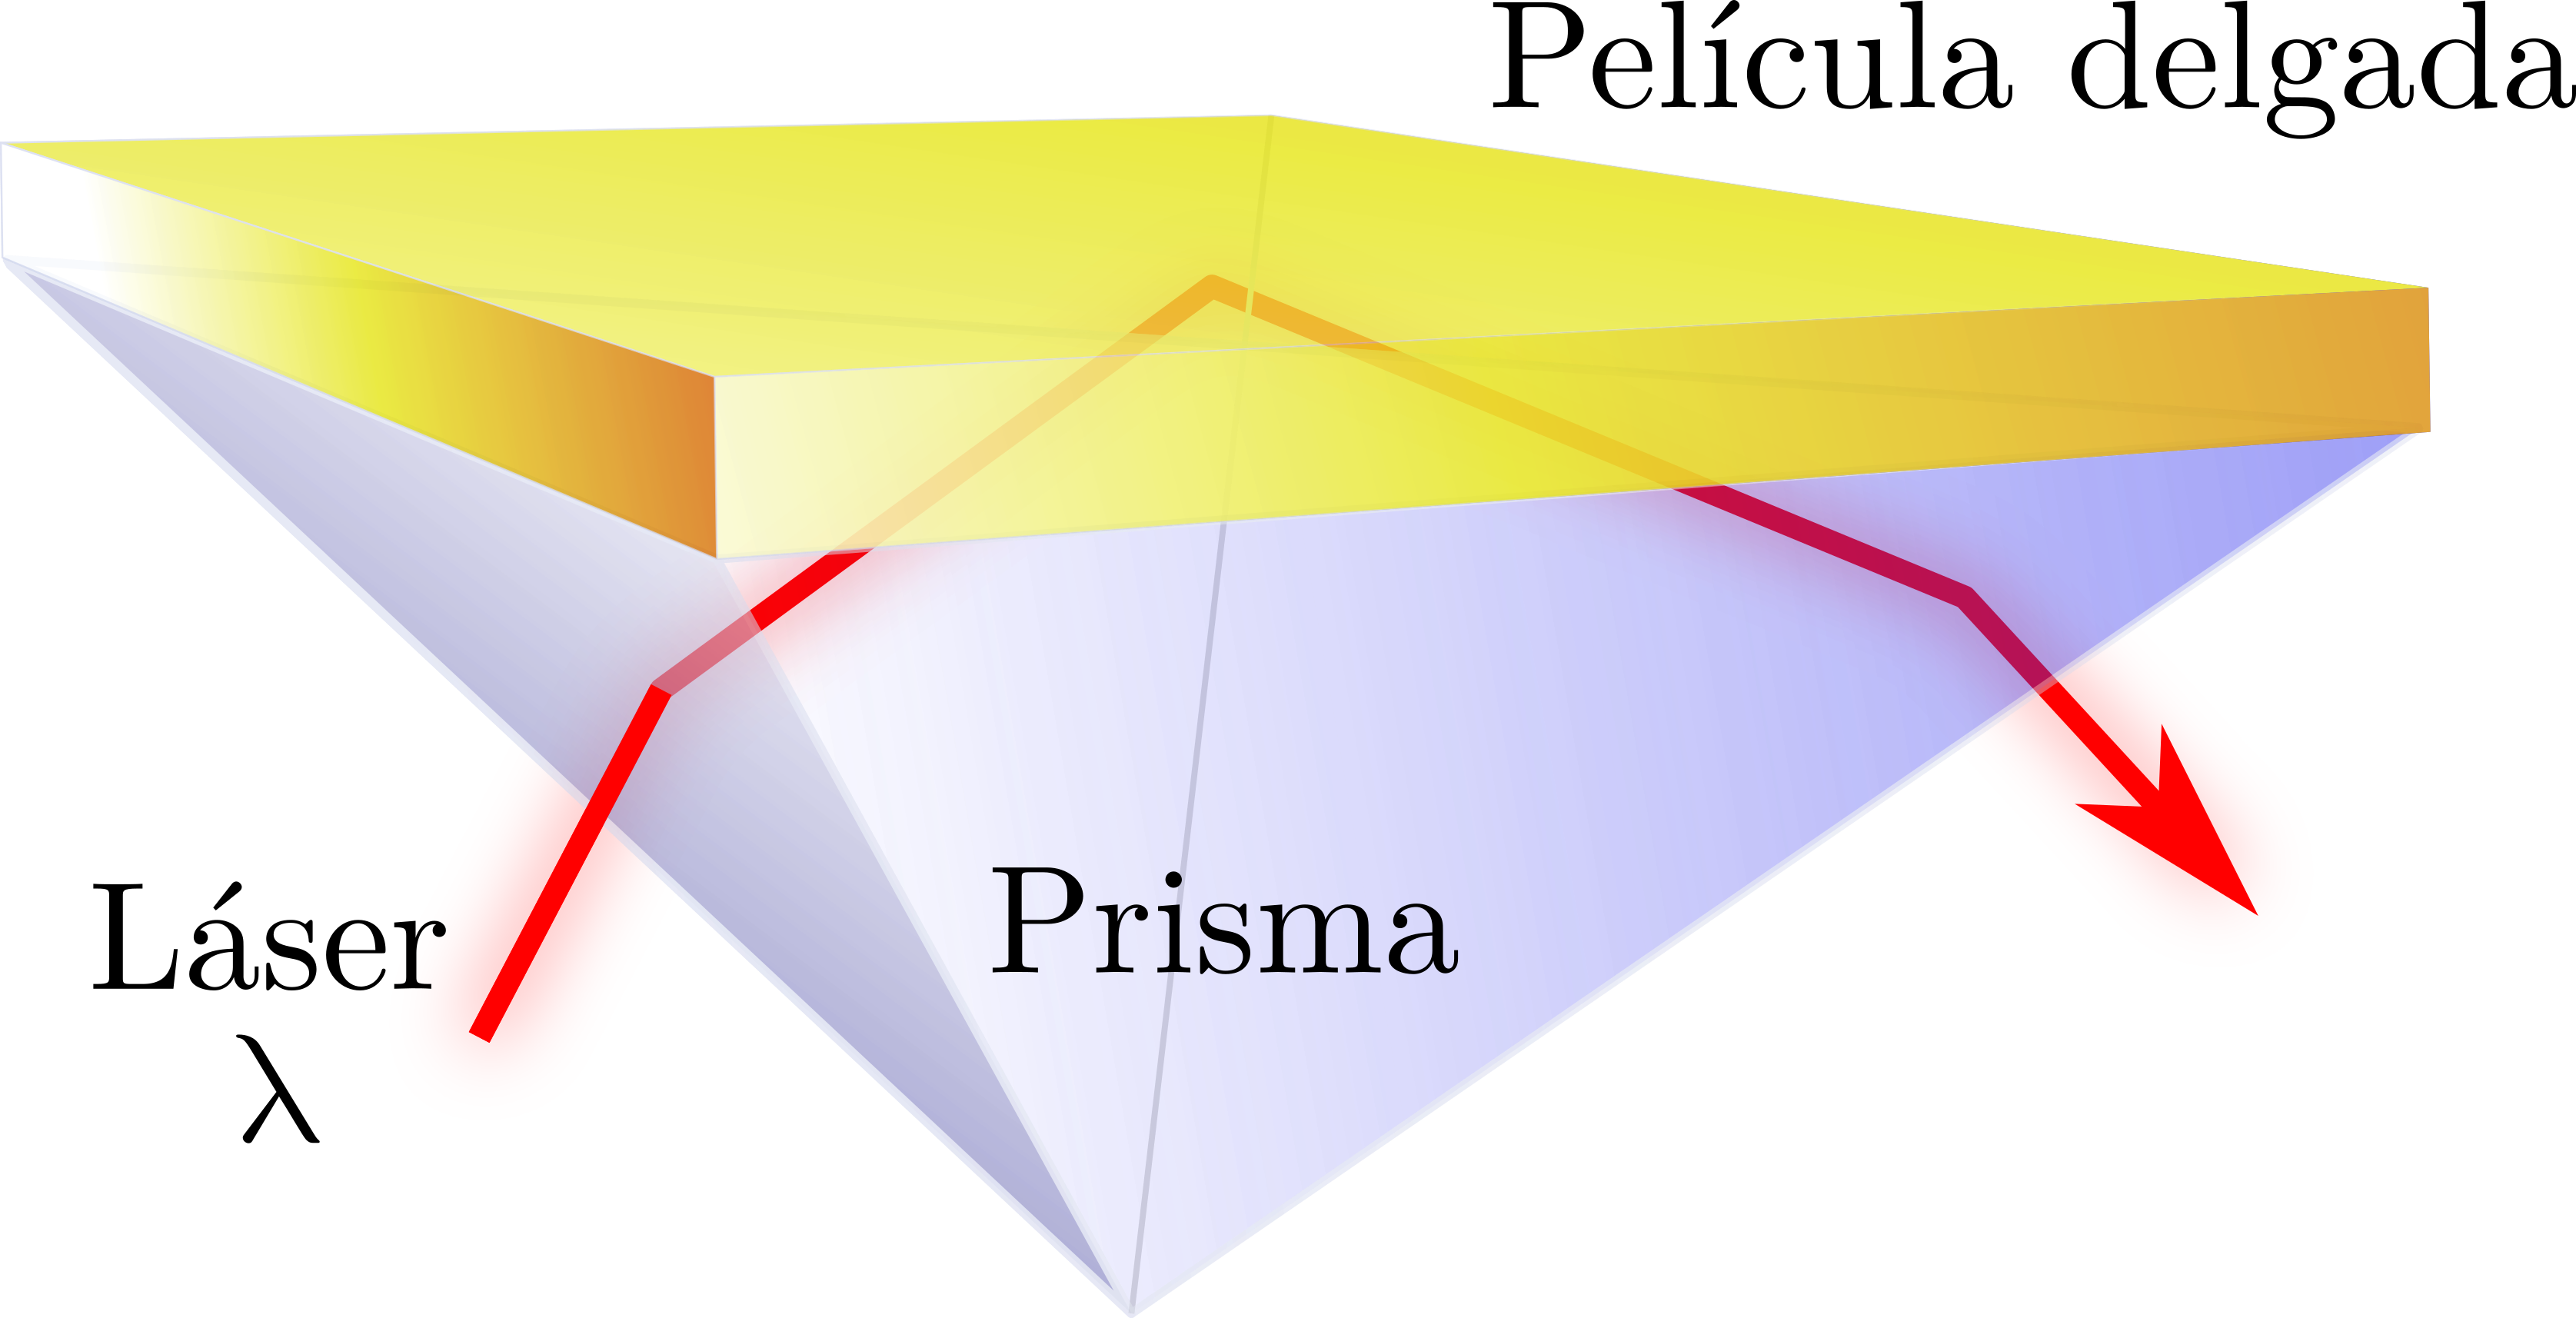
\includegraphics[scale=.225]{0-4-Introduccion/figs/SPP-3D.png}
		\end{subfigure}
	\begin{subfigure}{.05\textwidth}\vspace{-3.5cm}\caption{}\label{sfig:ATRNP}	\end{subfigure}
	\begin{subfigure}{.43\textwidth}  
		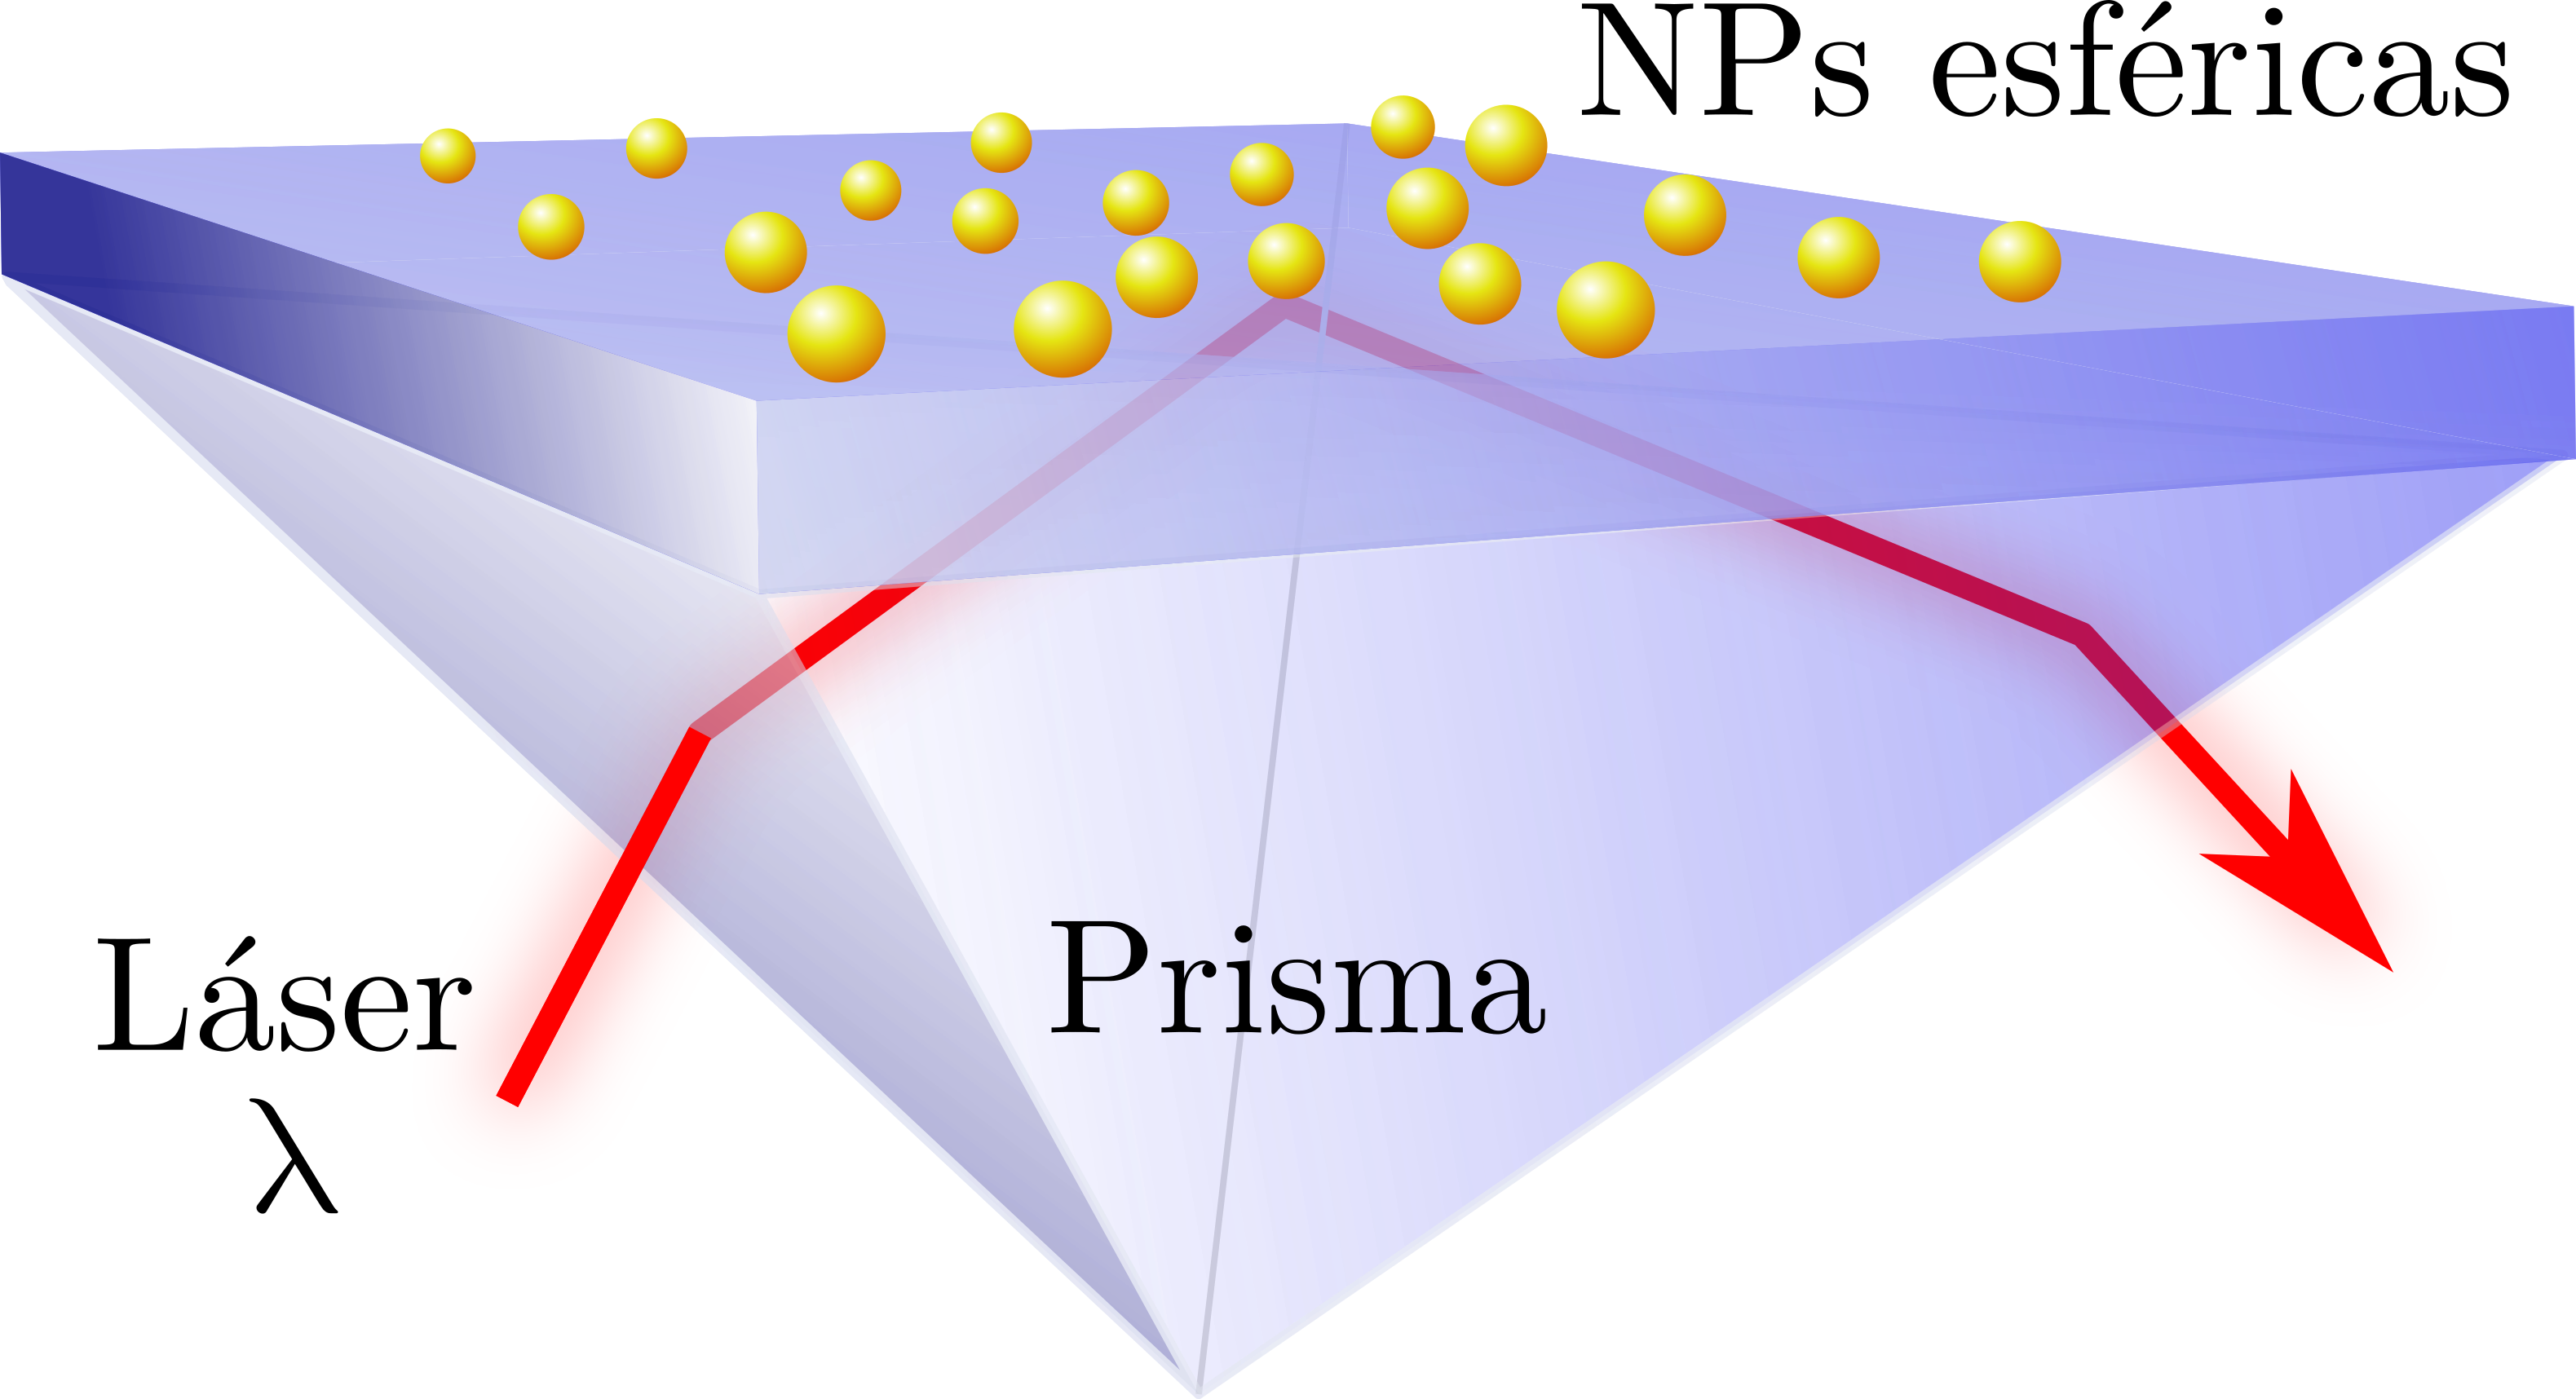
\includegraphics[scale=.225]{0-4-Introduccion/figs/NPs-3D.png}
	\end{subfigure} 
	\caption{ Iluminación de \textbf{a)} una película delgada y \textbf{b)} un arreglo de NPs esf\'ericas desordenadas por un haz óptico de longitud de onda $\lambda$, en configuraci\'on ATR.}	\label{fig:ATR1}	
	\end{figure}	
	
En el 2009 se public\'o un art\'iculo \cite{kabashin2009plasmonic} en el que se propone un sistema bidimensional de NPs cilíndricas de oro, localizadas periódicamente, para la mejora de la resoluci\'on  en el biosensado [ver Fig. \ref{sfig:Nanocilindros}]; las dimensiones de los nanocilindros y el parámetro de red del arreglo son menores que la longitud de onda con la que se ilumina el arreglo \cite{kabashin2009plasmonic}.  En el artículo se reportó un modo plasmónico distinto a los modos de las NPs individuales, que permite el sensado del índice de refracción de la matriz y se le denominó \textit{modo guiado} \cite{kabashin2009plasmonic}.  En el 2018 se publicó que este modo es una respuesta colectiva del arreglo periódico \cite{danilov2018ultra} y que depende del parámetro de red; en este artículo se le identificó como una \emph{resonancia de red de superficie plasmónica} (Plasmonic Surface Lattice Resonance, PSLR), las cuales ocurren cuando un rayo que se refracta por la estructura periódica excita una LSPR en los elementos de la estructura \cite{vakevainen2013plasmonic}; las PSLR dependen del  ángulo de incidencia y de la periodicidad del arreglo \cite{danilov2018ultra} y pueden acoplarse con la matriz o con el sustrato. En la Fig. \ref{sfig:DipATR} se reproducen las gráficas (extraídas de \cite{kabashin2009plasmonic}) de la reflectancia como función de la longitud de onda, para el arreglo mostrado en la Fig.  \ref{sfig:Nanocilindros}, en donde se consideró un sustrato de vidrio ($n=1.5$) y una matriz de aire ($n=1$), así como una monocapa de nanocilindros de $360$ nm de largo, $25$ nm de diámetro, con una separación entre ellos de $60$ nm. La respuesta EM del arreglo de nanocilindros   fue calculada al considerar a los cilindros como nanoesferoides y emplear una modificación del modelo de Maxwell Garnett \cite{atkinson2006anisotropic} ---que es una teoría de medio efectivo\footnote{Proceso de homogenización en donde se sustituye el medio heterogéneo por un medio continuo equivalente.  Este proceso se basa en la respuesta promedio del medio original cuando la longitud de onda de la luz incidente es grande en comparación a las dimensiones del sistema \cite{sihvola1999mixing}.}--- para la función dieléctrica efectiva de la monocapa $\varepsilon(\omega) = n^2 (\omega)$. En la Fig. \ref{sfig:k(w)Kobashin} se grafica la relación de dispersión  (energía como función de la  proyección perpendicular al sustrato del vector de onda) de la PSLR (puntos blancos), mientras que en la Fig.  \ref{sfig:dLambda} se grafican los resultados experimentales del corrimiento de la PSLR al cambiar el índice de refracción de la matriz (reproducida de \cite{danilov2018ultra}).

	\begin{figure}[h!]\centering
		\begin{subfigure}{.01\linewidth}\caption{ }\label{sfig:Nanocilindros} \vspace{5cm}	\end{subfigure}  
		\begin{subfigure}{.45\linewidth}\hspace*{-3em}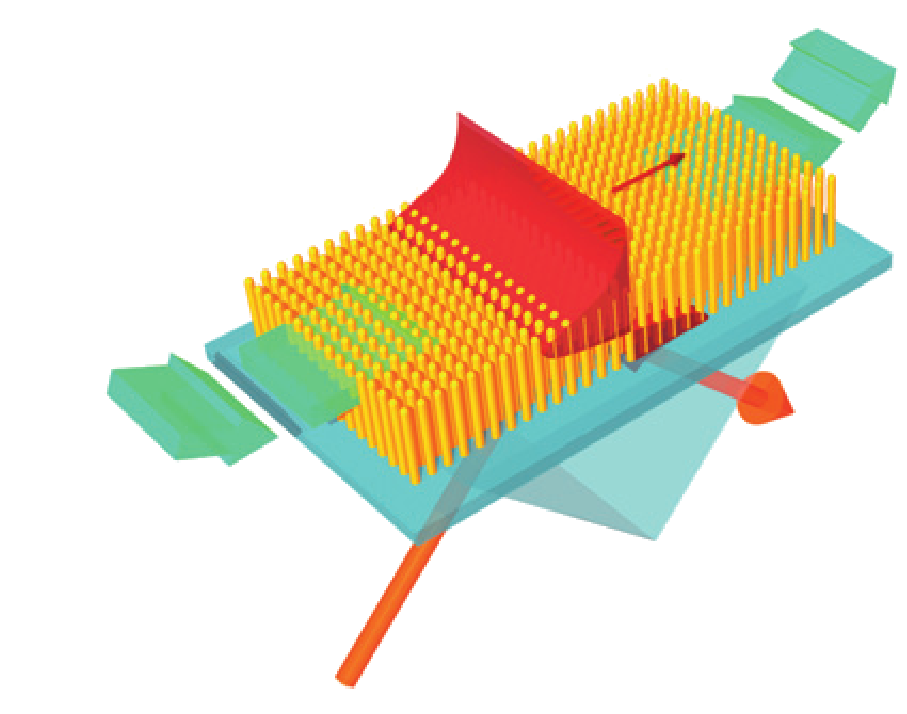
\includegraphics[scale=1]{0-4-Introduccion/figs/nanorods.png}\end{subfigure}
\begin{subfigure}{.01\linewidth}\caption{ }\label{sfig:DipATR}\vspace{4.75cm}\end{subfigure}  
		\begin{subfigure}{.45\linewidth}\hspace*{-1em}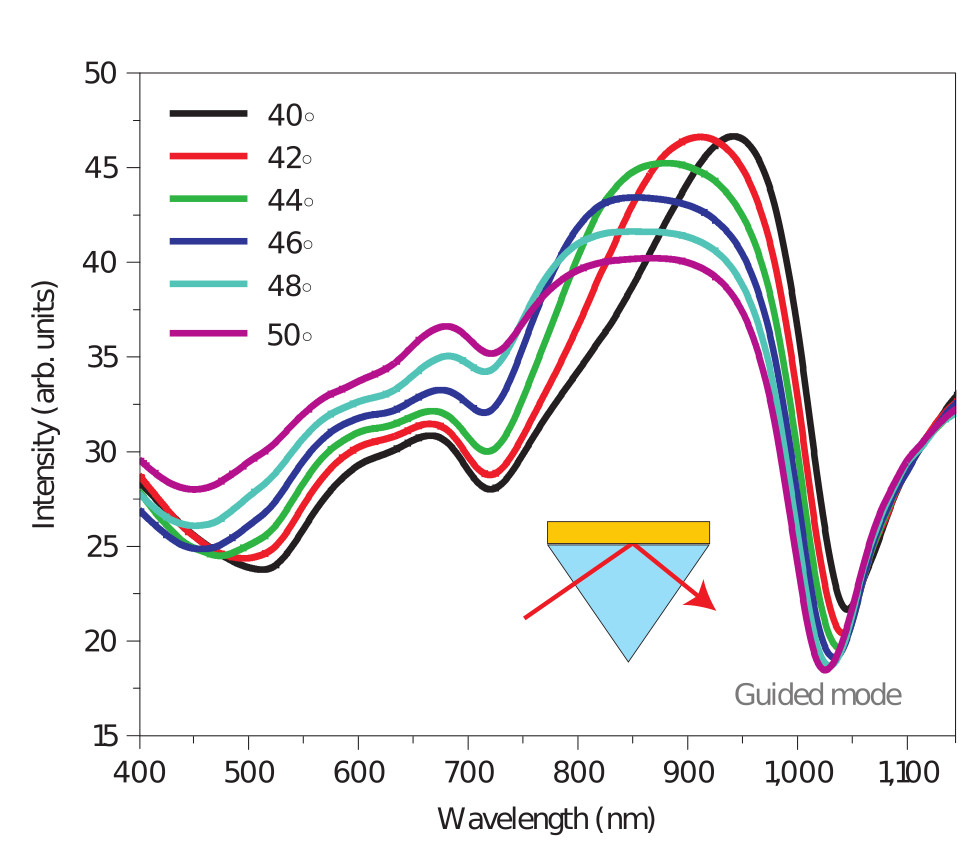
\includegraphics[scale=.9]{0-4-Introduccion/figs/reflectancia.png}\end{subfigure}\\
\begin{subfigure}{.01\linewidth}\caption{ }\label{sfig:k(w)Kobashin} \vspace{5cm}	\end{subfigure} 
		\begin{subfigure}{.45\linewidth}\hspace{1em}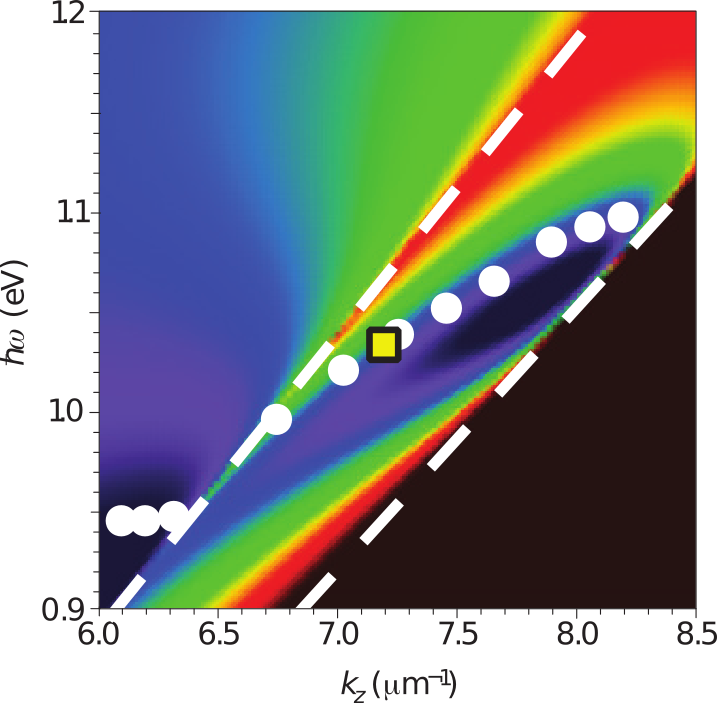
\includegraphics[scale=1]{0-4-Introduccion/figs/dispersion.png}\end{subfigure}	
\begin{subfigure}{.01\linewidth}\caption{ }\label{sfig:dLambda}\vspace{4.75cm}\end{subfigure}  
		\begin{subfigure}{.45\linewidth}\hspace*{-.5em}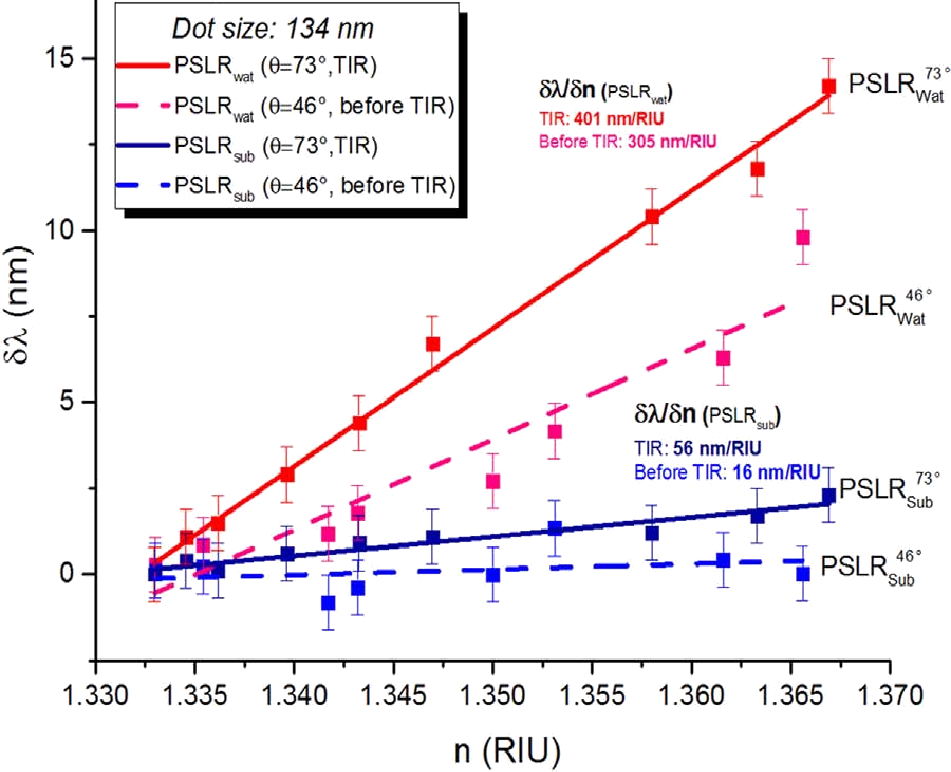
\includegraphics[scale=.9]{0-4-Introduccion/figs/sensibilidad.png}\end{subfigure}		
		\caption{\textbf{a)} Esquema de  un arreglo periódico cuadrado de nanocilindros de oro ---extraído de  \cite{kabashin2009plasmonic}---. \textbf{b)} Cálculos de la reflectancia ---extraídos de  \cite{kabashin2009plasmonic}--- como función de la longitud de onda $\lambda$, para distintos ángulos de incidencia, y \textbf{c)} de la relación de dispersión ---extraída de  \cite{kabashin2009plasmonic}---, considerando nanocilindros inmersos en una matriz de aire ($n=1$), sobre un sustrato de vidrio ($n=1.5$), de $360$ nm de largo, $25$ nm de diámetro y una separación de $60$ nm entre ellos. En \textbf{d)} se grafican los resultados experimentales ---extraídos de  \cite{danilov2018ultra}--- del corrimiento de las PSLR excitadas para un arreglo de nanocilindros inmersos en agua y soportados por un sustrato de vidrio para un ángulo de incidencia de $46^\circ$ y $73^\circ$; para este caso se emplearon cilindros de altura de $90$ nm, de diámetro de $134$ nm y una separación de $320$ nm. Las mediciones se realizaron cuando las oscilaciones del plasmón se acoplan con la matriz (PSLR$_{H_2{O}}$) y con el sustrato (PSLR$_{sus}$).}\label{fig:GraphsPapersNANOCILINDROS}
	\end{figure}

Los cálculos de la reflectancia en ATR [Fig. \ref{sfig:DipATR}], muestran las resonancias plasmónicas típicas de NPs individuales para cilindros (modo longitudinal alrededor de $720$ nm y el transversal alrededor de $500$ nm) y adicional a ellas, se observa la PSLR alrededor de los $1,050$ nm. La PSLR, al excitarse a energías menores del modo longitudinal, no puede corresponder a una resonancia de NP individual y por tanto debe corresponder a un modo colectivo. En la Fig.  \ref{sfig:k(w)Kobashin} se grafica la relación de dispersión de dicho modo, donde los puntos blancos corresponden a los mínimos en la reflectancia alrededor de $1,050$ nm de la Fig.  \ref{sfig:DipATR} de la PSLR.  Las líneas punteadas en la Fig.   \ref{sfig:k(w)Kobashin} corresponden a los ángulos críticos de las interfaces del medio efectivo simulado con el aire (línea superior izquierda) y con el sustrato (línea inferior derecha); la región oscura debajo de la línea punteada inferior derecha representa las combinaciones de energía y vector de onda sin sentido físico\footnote{La proyección del vector de onda perpendicular a la interfaz está dada por $k_z = (\omega / c)n_m\cos\theta_i$, donde $\omega$ y $\theta_i$ son la frecuencia angular y el ángulo de incidencia de la onda plana incidente, respectivamente. La combinación de $\hbar\omega$ y $k_z$ en la región negra de la Fig. \ref{sfig:k(w)Kobashin} corresponde a valores donde $\cos\theta_i>1$, dando como resultado un ángulo complejo de incidencia, por lo que no tiene sentido físico.}.  En la Fig.  \ref{sfig:dLambda} se muestra el corrimiento de la longitud de onda de excitación $\delta\lambda$ de las PSLRs como función del índice de refracción de la matriz $n$ ---medido en unidades de índice de refracción (Refractive Index Units, RIU)--- cuando un haz de luz que incide a $46^\circ$ (líneas punteadas) y  a $73^\circ$ (líneas sólidas) se difracta por la matriz de agua (líneas roja y magenta) y por el sustrato de vidrio (líneas azul y morado). Dentro de la gráfica se muestran los valores de la sensibilidad $\delta \lambda/\delta n$ para cada caso.  

%\section*{Planteamiento del problema}

Los biosensores basados es nanoestructuras periódicas ordenadas, como el de nanocilindros mostrado en la Fig. \ref{sfig:Nanocilindros}, pueden ser sintonizados a una longitud de onda particular al ajustar el parámetro de red del arreglo, permitiendo optimizar la medición del sensor para cada tipo de muestra, además de ser compatibles con equipos comerciales actuales \cite{kabashin2009plasmonic}.  Sin embargo, la fabricaci\'on de arreglos ordenados de NPs presenta una complicaci\'on t\'ecnica de alto costo y largo tiempo de fabricación \cite{estevez2014trends}, por lo que en esta tesis se propone el uso de un arreglo bidimensional desordenado de NPs esféricas que presente una respuesta colectiva semejante a la reportada en \cite{kabashin2009plasmonic} y \cite{danilov2018ultra}. Se ha observado que la respuesta colectiva en un arreglo desordenado también es sintonizable según las propiedades de las NPs empleadas, por lo que su uso en sensado no sólo cuenta con las ventajas de los sensores propuestos en \cite{kabashin2009plasmonic} y \cite{danilov2018ultra}, sino también una reducción en los precios y tiempos de fabricación. 

%\section*{Metodología}
Para  caracterizar la respuesta óptica de un arreglo bidimensional desordenado de NPs esféricas plasmónicas se emplea el modelo de esparcimiento coherente (Coherent Scattering Model, CSM) \cite{reyes2018analytical}, el cual proporciona expresiones analíticas para los coeficientes de amplitud de reflexión y de transmisión para una monocapa de NPs esféricas, idénticas, y desordenadas.  Las expresiones  dadas por el CSM dependen de las componentes de la matriz de esparcimiento que aparece en la solución de Mie ---que resuelve los campos EMs esparcidos por una esfera iluminada por una onda plana monocromática \cite{bohren1998absorption}---, así como la respuesta EM del material con que están hechas las partículas esféricas de la monocapa: la función dieléctrica $\varepsilon(\omega)$.  Para caracterizar una excitación equivalente a la PSLR estudiada en \cite{kabashin2009plasmonic} y \cite{danilov2018ultra}, es decir, una respuesta colectiva apta para el biosensado, se calcula la reflectancia y transmitancia del sistema monocapa mediante los coeficientes de amplitud de reflexión y transmisión del CSM. 
 
Adicional a la caracterización de la respuesta óptica de una monocapa desordenada de NPs esféricas e idénticas dada por el CSM, se realiza una comparación entre ésta y la respuesta óptica de los biosensores comerciales basados en SPPs. La comparación se realiza mediante un análisis de sensibilidad (el corrimiento de la longitud de onda de la resonancia respecto al cambio del índice de refracción de la matriz $\delta\lambda_{res}/\delta n$) y de la \emph{figura de mérito} (Figure Of Merit, FoM) de bulto $\textit{FoM}_B$ ---definida como $(\delta\lambda_{res}/\delta n)/\Gamma$, con $\Gamma$ la anchura a media altura (Full Width at Half Maximum, FWHM)---, como se  efectúa en \cite{svedendahl2009refractometric}, donde se compara experimentalmente la respuesta óptica de una monocapa desordenada de nanodiscos (NDs)  de oro [ver Fig. \ref{sfig:NanoDisks}] con la de una película continua de oro. Los NDs empleados en \cite{svedendahl2009refractometric} son nanocilindros de $30$ nm de altura y  $120$ nm de diámetro\footnote{En \cite{svedendahl2009refractometric} no se da información sobre la fracción de cubierta ni de la distancia mínima promedio entre NDs.}, mientras que el grosor de la película continua es de $50$ nm: estos parámetros sintonizan la LSPR de los ND y el SPP a $700$ nm, considerando $\theta_i=70^\circ$. En la Fig. \ref{sfig:TNanoD} se grafica la longitud de onda de resonancia  $\lambda_{res}$ del arreglo desordenado de NDs, que coincide con la LSPR de los nanocilindros individuales, como función del ángulo de incidencia $\theta_i$; los valores de $\lambda_{res}$ corresponden a los mínimos de la transmitancia graficada en el recuadro dentro de la Fig. \ref{sfig:TNanoD}. En la Fig. \ref{sfig:resumenNDs} \textbf{i)} se grafican la reflectancia y la transmitancia  en una configuración de iluminación directa del arreglo desordenado de NDs, mientras que en la Fig. \ref{sfig:resumenNDs} \textbf{ii)} se grafica la reflectancia, en configuración ATR, para la película continua de oro, en ambos caso se considera una matriz de agua ($n=1.33$) y de agua con distintas concentraciones de etilenglicol. Finalmente, en la Fig. \ref{sfig:resumenNDs} \textbf{iii)} se grafica el corrimiento de la resonancia $\delta\lambda_{res}$ como función del índice de refracción de la matriz; la sensibilidad tanto del SPP como la LSPR de los NDs se muestran dentro de la gráfica. A partir de la Fig. \ref{sfig:resumenNDs} se concluye en \cite{svedendahl2009refractometric} que la sensibilidad del SPP ($3,300$ nm~\mbox{RIU$^{-1}$}) es mayor a la del arreglo desordenado de NDs ($178$ nm~\mbox{RIU$^{-1}$}), lo cual también ocurre con las FoM: para el SPP se obtiene que $\textit{FoM}_{B,\textit{SPP}}\approx 57 \mbox{ RIU$^{-1}$}$, mientras que para los ND $\textit{FoM}_{B,\textit{ND}}\approx 2\mbox{ RIU$^{-1}$}$. Los resultados reportados en \cite{svedendahl2009refractometric} para la sensibilidad y la $\textit{FoM}_B$ son consistentes con lo reportado en la literatura \cite{brian2009sensitivity,cahill1997surface}.
 
\begin{figure}[t!]\centering
\begin{minipage}[c]{.48\linewidth}
		\begin{subfigure}{.01\linewidth}\caption{ }\label{sfig:NanoDisks} \vspace{4.cm}	\end{subfigure}  
		\begin{subfigure}{.98\linewidth}\hspace*{3em}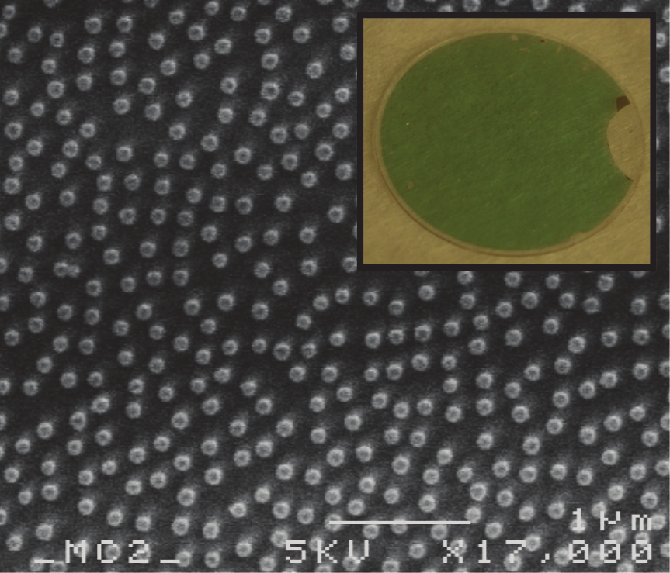
\includegraphics[scale=1.]{0-4-Introduccion/figs/nanoDisk.png}\end{subfigure}\\
\noindent \begin{subfigure}{.01\linewidth}\caption{ }\label{sfig:TNanoD}\vspace{3.5cm}\end{subfigure}  
		\begin{subfigure}{.98\linewidth}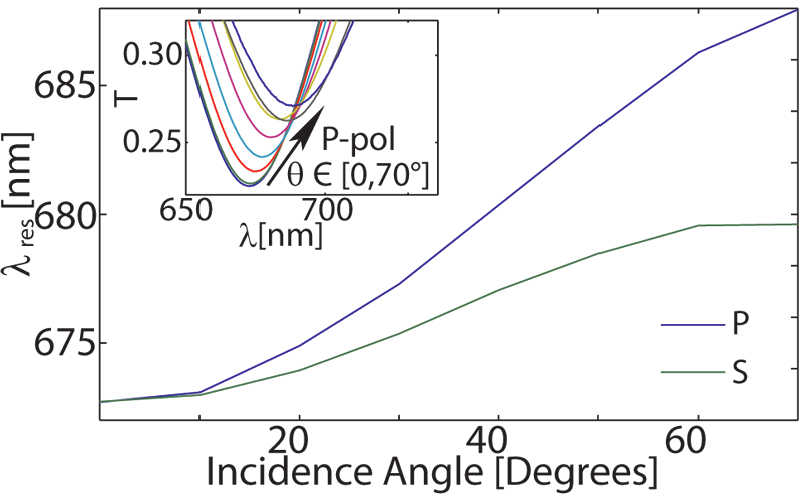
\includegraphics[scale=1.1,trim={0 0 0 -1em},clip]{0-4-Introduccion/figs/TransmitanciaND.png}\end{subfigure}
\end{minipage}		
		\begin{subfigure}{.01\linewidth}\caption{ }\label{sfig:resumenNDs} \vspace{9cm}	\end{subfigure} 
		\begin{subfigure}{.48\linewidth}\hspace{.5em}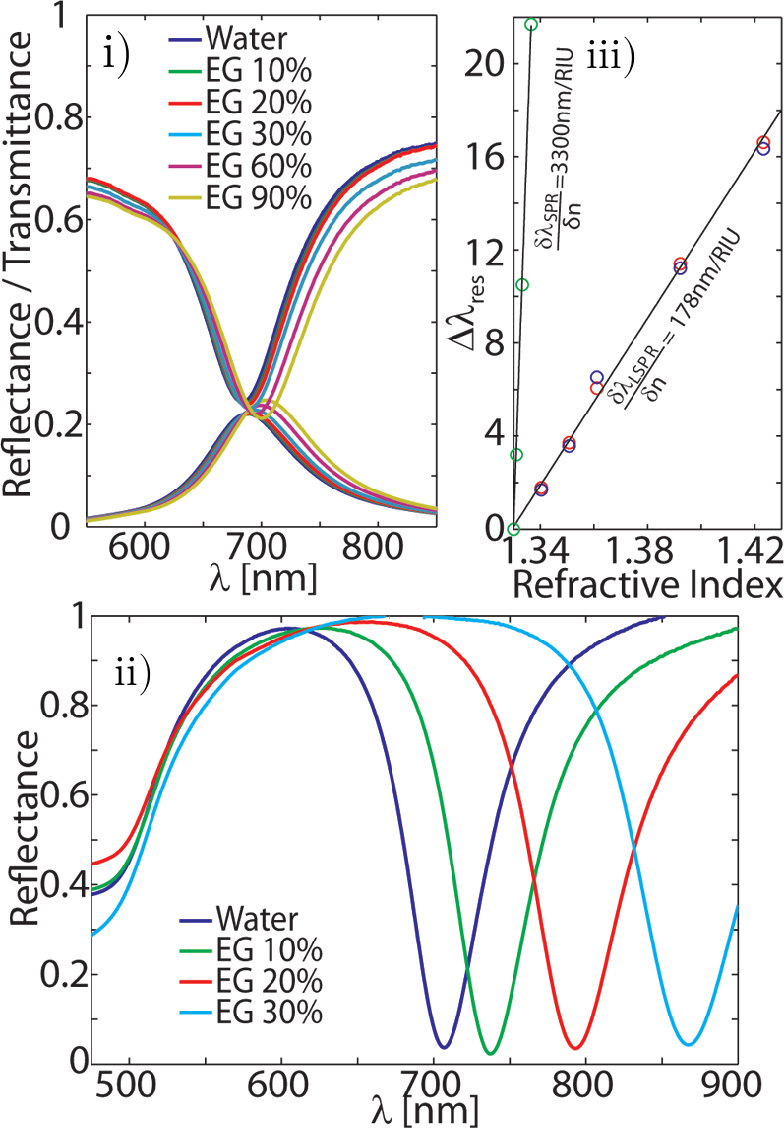
\includegraphics[scale=1.05]{0-4-Introduccion/figs/resumenND.png}\end{subfigure}		
		\caption{ \textbf{a)} Micrografía de electrones de barrido de la muestra del arreglo desordenado de NDs ---nanocilindros de $30$ nm de altura y  $120$ nm de diámetro--- de oro sobre vidrio. El recuadro interior muestra una fotografía de la muestra con un sustrato de $2.5$ cm de diámetro. \textbf{b)} Gráfica de la longitud de onda de resonancia $\lambda_{res}$ del arreglo desordenado de NDs como función del ángulo de incidencia para ambas polarizaciones: \emph{s} y \emph{p}. Los valores de $\lambda_{res}$ corresponden a los mínimos de la transmitancia graficada dentro del recuadro. \textbf{c)} Gráfica \textbf{i)} de la transmitancia y reflectancia del arreglo de NDs en iluminación directa y \textbf{ii)} de la reflectancia de una película delgada de oro de $50$ nm de grosor en una configuración ATR como función de la longitud de onda $\lambda$, considerando una matriz de agua ($n=1.33$) y de agua con distintas concentraciones  de etilenglicol; \textbf{iii)} corrimiento de $\lambda_{res}$ presente en la película delgada y en el arreglo de NDs; el valor de la sensibilidad de cada arreglo se encuentra dentro de la gráfica. Todas las gráficas fueron extraídas de \cite{svedendahl2009refractometric}.}\label{fig:GraphsPapersNANODISKS}
	\end{figure} 
 
El objetivo de esta tesis de licenciatura es caracterizar la respuesta EM de una monocapa desordenada de NPs esféricas idénticas soportada por un sustrato, calculando la reflectacia y transmitancia de forma analítica por el formalismo del CSM (considerando monocapas formadas por NPs de oro y de plata), y compararla tanto con la de una película continua de $50$ nm de grosor (sistema empleado en biosensores comerciales) \cite{svedendahl2009refractometric}, como con la de una monocapa de nanocilindros ordenados \cite{kabashin2009plasmonic,danilov2018ultra} y con la de una monocapa de nanodiscos desordenados \cite{svedendahl2009refractometric}, y evaluar si el sistema de NPs esféricas desordenadas es apto para el biosensado.

Para determinar si una monocapa desordenada de nanopartículas esféricas puede ser empleada como biosensor, se realizaron cálculos de la reflectancia en ATR para una monocapa de NPs embebidas en agua y soportadas por un sustrato de vidrio, considerando que la función dieléctrica de las NPs en la monocapa está dada por el modelo de Drude-Sommerfeld. Se caracterizó un modo plasmónico distinto a las SPRs de partículas individuales mediante variaciones del radio de las NPs y de la fracción de cubierta de las monocapa. Es decir, primero se estudió el supuesto modo plasmónico colectivo para una monocapa de NPs ideales, y posteriormente se estudiaron monocapas con NPs de materiales reales: oro y plata. Mediante la caracterización, variando nuevamente el radio de las NPs de la monocapa y la fracción de cubierta de ésta, se determinaron los parámetros óptimos para que las monocapas de NPs de oro y de plata sean propuestas como biosensores. Finalmente, se comparó la sensibilidad del supuesto modo plasmónico colectivo ante cambios en el índice de refracción de la matriz donde están embebidas las NPs con la sensibilidad del SPP excitado en una película continua de oro de $50$ nm (sensores comerciales) y con propuestas de arreglos nanoestructurados para el biosensado publicados en \cite{kabashin2009plasmonic,danilov2018ultra,svedendahl2009refractometric}; asimismo se calcularon las FoM de bulto para el supuesto modo plasmónico colectivo y para el SPP considerado tanto oro como plata para las NPs en la monocapa y para la película continua.

Esta tesis está dividida en tres partes: Teoría (capítulo \ref{chapter:Teoria}), Respuesta óptica de una monocapa desordenada de nanopartículas esféricas (capítulo \ref{chapter:Resultados}) y Conclusiones. En el capítulo \ref{chapter:Teoria}, se presentan en la sección \ref{section:NocionesBasicas} la solución tipo ondas planas de las ecuaciones de Maxwell y las ecuaciones de Fresnel para describir el comportamiento de una onda plana monocromática al incidir sobre una superficie plana entre dos medio materiales lineales, homogéneos e isótropos, mientras que en la sección \ref{section:Mie} se estudia la solución de Mie, que resuelve las ecuaciones de Maxwell para una partícula esférica, empleando la matriz de esparcimiento que relaciona los campos EMs esparcidos por la esfera con los campos EMs incidentes, explicando el problema de absorción y esparcimiento de luz por una partícula esférica de material y tamaño arbitrario. En la sección \ref{section:RespuestaEM} se estudia la respuesta EM de materiales plasmónicos en bulto y a escala nanométrica: en la subsección \ref{ssection:Drude} se presenta el modelo de Drude-Sommerfeld (respuesta EM de un gas de electrones libres) para la función dieléctrica, mientras que en la sección \ref{ssection:CorreccionTamano} se presenta un método para determinar los parámetros del modelo de Drude-Sommerfeld que ajustan a los datos experimentales de la función dieléctrica del oro y de la plata, así como una corrección por tamaño de la función dieléctrica para NPs esféricas; asimismo, en la sección \ref{ssection:Plasmones} se presentan los plasmones, que son oscilaciones colectivas resultado del acoplamiento entre una onda plana y los electrones libres de algún material. En la  sección \ref{section:CSM} se estudia el CSM, que proporciona expresiones analíticas para los  coeficientes de amplitud de reflexión y de transmisión de una monocapa desordenada de NPs esféricas e idénticas, suspendida en el espacio libre (sección \ref{ssection:FSM}) y  soportada por un sustrato (sección \ref{ssection:CSMATR}), cuando una onda plana monocromática incide sobre la monocapa. Posteriormente, en el capítulo \ref{chapter:Resultados}, se presentan en la sección \ref{section:Drude} los resultados de la reflectancia de una monocapa de NPs con una función dieléctrica tipo Drude, suspendida en el espacio libre (subsección \ref{ssection:DrudeFSM}) y soportada por un sustrato e iluminada en una configuración ATR (subsección \ref{ssection:DrudeATR}). En la sección \ref{section:AuAg} se presentan los resultados de la reflectancia en una configuración ATR de una monocapa de NPs de oro y de plata y en la sección \ref{section:sensLambda} se realiza un análisis de sensibilidad para una monocapa de NPs esféricas de oro y se compara con la de una película continua de oro $50$ nm de grosor y con la propuestas de sistemas nanoestructurados. Por último, se escriben las conclusiones, con base en los resultados del capítulo \ref{chapter:Resultados}, para el posible empleo de una monocapa de NPs de oro y de plata como biosensor, así como trabajo a futuro.
